\documentclass[10pt]{beamer}

\usetheme{metropolis}
\usepackage{appendixnumberbeamer}

\usepackage{booktabs}
\usepackage[scale=2]{ccicons}
\usepackage{graphicx}
\usepackage{hyperref}
\usepackage{circuitikz}
\usepackage{pdflscape}
\usepackage{smartdiagram}

\usepackage{color}
\usepackage{listings}

\lstset{
	basicstyle=\footnotesize\ttfamily,
    keepspaces=true,
    showstringspaces=false,
    language=PHP,
    commentstyle=\ttfamily,
}

\usepackage[OT4]{polski}
\usepackage[utf8]{inputenc}

\usepackage{pgfplots}
\usepgfplotslibrary{dateplot}

\usepackage{xspace}
\newcommand{\themename}{\textbf{\textsc{metropolis}}\xspace}

\setbeamertemplate{frame footer}{}
\setbeamertemplate{frame numbering}{}

\usetikzlibrary{shapes,arrows}

\tikzstyle{decision} = [diamond, draw, fill=blue!20, 
    text width=4.5em, text badly centered, node distance=3cm, inner sep=0pt]
\tikzstyle{block} = [rectangle, draw, fill=blue!20, 
    text width=5em, text centered, rounded corners, minimum height=4em]
\tikzstyle{line} = [draw, -latex']
\tikzstyle{cloud} = [draw, ellipse,fill=red!20, node distance=3cm,
    minimum height=2em]


\title{Mechanizmy pamięci podręcznej i optymalizacja}

\subtitle{Projektowanie i programowanie systemów internetowych I}
\author{mgr inż. Krzysztof Rewak}
\date{\today}
\institute{Wydział Nauk Technicznych i Ekonomicznych \\ Państwowa Wyższa Szkoła Zawodowa im. Witelona w Legnicy}

\begin{document}

\maketitle

\begin{frame}{Plan prezentacji}
  \setbeamertemplate{section in toc}[sections numbered]
  \tableofcontents[hideallsubsections]
\end{frame}


\section{Pamięć podręczna}

\begin{frame}{Z definicji}
	Uogólniając, \textbf{pamięć podręczna} to pamięć o krótszym czasie dostępu niż standardowo wykorzystywana pamięć.
\end{frame}

\begin{frame}{Z definicji}
	Podstawowym celem wykorzystania pamięci podręcznej jest zatem zwiększenie szybkości dostępu do \emph{pewnych} danych.
\end{frame}

\begin{frame}{\emph{Pewne dane?}}
	Jakie informacje powinny być przechowywane w pamięci podręcznej?
	
	Dowolne. \ \\ \ \\ \ \\ \ \\
\end{frame}

\begin{frame}{\emph{Pewne dane?}}
	Jakie informacje powinny być przechowywane w pamięci podręcznej?
	
	Dowolne, ale najsensowniejszym wyjściem jest przechowywanie danych, które najprawdopodobniej według wybranych wskaźników będą wykrozystane w najbliższym czasie.
\end{frame}

\begin{frame}{Gdzie można znaleźć pamięć podręczną?}
	\begin{itemize}
		\item procesor
		\item dysk twardy
		\item system plików
	\end{itemize}
\end{frame}

\begin{frame}{Gdzie można znaleźć pamięć podręczną?}
	\begin{itemize}
		\item przeglądarka internetowa
		\item pomiędzy przeglądarką a serwerem HTTP
		\item bazy danych
	\end{itemize}
\end{frame}

\section{Cache przeglądarki internetowej}

\begin{frame}{Okno na internet}
	Przeglądarka internetowa służy do łączenia się poprzez protokół HTTP(S) z serwerem i wyświetlania jego odpowiedzi. Umożliwia również interakcję z serwerem w sposób zaprojektowany przez programistę.
\end{frame}

\begin{frame}{Okno na internet}
	Korzystając z narzędzi deweloperskich łatwo można podejrzeć ile zapytań wykonuje wejście na dowolną stronę w internecie.
\end{frame}

\begin{frame}{Pod maską}
	\begin{figure}[t]
		\centering
		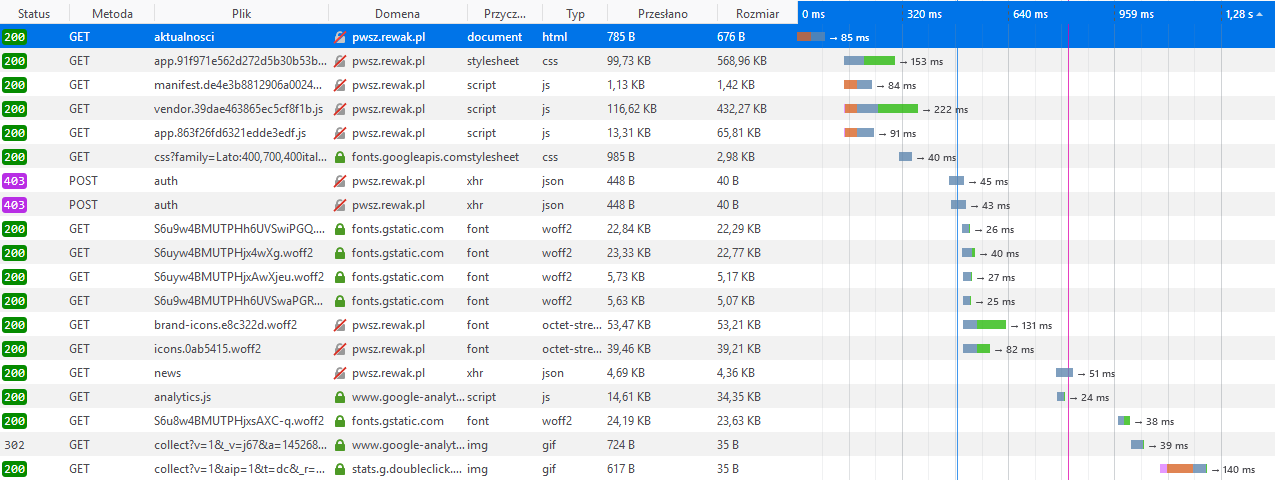
\includegraphics[width=\linewidth]{f122.png}
	\end{figure}
\end{frame}

\begin{frame}{Pod maską}
	Kolejno wczytywane są:
	\begin{itemize}
		\item strona \texttt{/aktualnosci}, czyli HTML
		\item załączone w HTML-u skrypty JS i style CSS
		\item odpytanie o status uwierzytelnienia
		\item fonty, ikony
		\item odpytanie o listę aktualności
		\item zewnętrzy skrypt Google Analytics
		\item odpytania do Google Analytics
	\end{itemize}
\end{frame}

\begin{frame}{Pod maską}
	Po odświeżeniu strony (F5) widać, że lista się zmniejszyła:
\end{frame}

\begin{frame}{Pod maską}
	\begin{figure}[t]
		\centering
		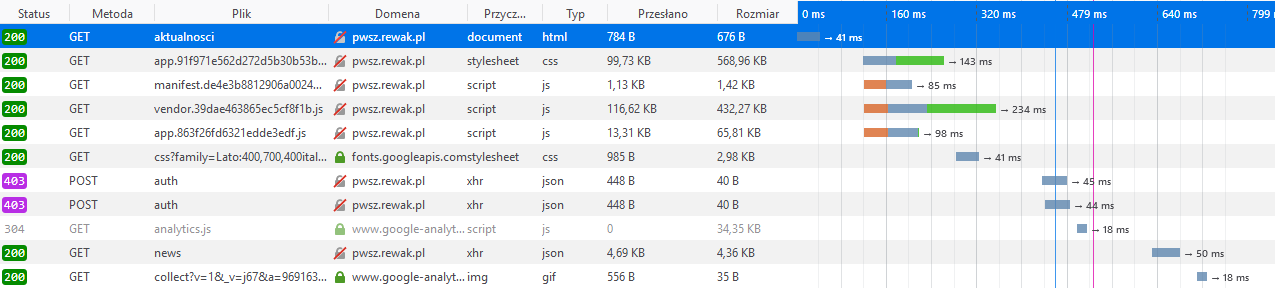
\includegraphics[width=\linewidth]{f12.png}
	\end{figure}
\end{frame}

\begin{frame}{Pod maską}
	Kolejno wczytywane są tym razem:
	\begin{itemize}
		\item strona \texttt{/aktualnosci}, czyli HTML
		\item załączone w HTML-u skrypty JS i style CSS
		\item odpytanie o status uwierzytelnienia
		\item odpytanie o listę aktualności
		\item zewnętrzy skrypt Google Analytics
		\item odpytania do Google Analytics
	\end{itemize}
\end{frame}

\begin{frame}{Co się stało?}
	Przeglądarka jest w stanie zapamiętać jaka strona prosiła o jakie zasoby. Pewne pliki mogą zostać zapisane w pamięci komputera, aby w przyszłości nie było wymagane pobieranie ich na nowo z internetu.
\end{frame}

\begin{frame}{Co cache'ować?}
	Do \emph{cache} trafiają najczęściej arkusze stylów, skrypty, fonty i grafiki.
\end{frame}

\begin{frame}{\emph{Nowy wspaniały świat}}
	W idealnie skonstruowanym frontendzie zapamiętane zostałyby zatem również:
	\begin{itemize}
		\item wszystkie załączone w HTML-u skrypty JS i style CSS
		\item zewnętrzy skrypt Google Analytics
	\end{itemize}
	
	aby odpytania wyglądały następująco:
	\begin{itemize}
		\item strona \texttt{/aktualnosci}, czyli HTML
		\item odpytanie o status uwierzytelnienia
		\item odpytanie o listę aktualności
		\item odpytania do Google Analytics
	\end{itemize}
\end{frame}

\begin{frame}{Zawsze?}
	Czy wszystkie wcześniej wymienione zasoby powinny zawsze być umieszczane w pamięci podręcznej przeglądarki?
	
	Można wykorzystać nagłówek \texttt{Cache-Control: no-cache} zapytania HTTP, aby ograniczyć \emph{cache'owanie} zasobów.
\end{frame}

\begin{frame}{\emph{Tips'n'tricks}}
	Kombinacja klawiszy Ctrl+F5 zazwyczaj czyści pamięć podręczna przeglądarki na aktualnie wyświetlanej stronie.
\end{frame}

\section{Cache HTTP}

\begin{frame}{Pośrednik HTTP}
	Pośredniczenie HTTP nie jest \emph{de iuro} systemem pamięci podręcznej, ale działa w podobny sposób.
\end{frame}

\begin{frame}{Pośrednik HTTP}
	Idea polega na rozmieszczeniu serwerów w taki sposób, aby informacje były przesyłane klientowi z najbliższego (również geograficznie!) serwera pośredniczącego.
\end{frame}

\begin{frame}{CDN}
	Na takiej zasadzie działają CDN-y, (ang. \emph{Content Delivery Network}), czyli rozproszone systemy dostarczania treści. Na takich serwerach przetrzymuje się przede wszystkim pliki CSS, JS i wszelakie pliki graficzne.
\end{frame}

\begin{frame}{CDN}
	Przykładowy link do biblioteki jQuery hostowanej na Cloudflare Amazonu:
	
	\texttt{https://cdnjs.cloudflare.com/ajax/libs/jquery/3.3.1/core.js}
\end{frame}

\section{Cache bazy danych}

\begin{frame}{\emph{Cache} danych}
	Pamięć podręczna może również zostać wykorzystana po stronie backendu, a najczęściej używana jest przy optymalizacji względem czasu pobierania danych. 
\end{frame}

\begin{frame}{Redis}
	Ilustrującym przykładem będzie aplikacja korzystająca bazowo z relacyjnej bazy danych MySQL, ale \emph{cache'ująca} pewne wyniki za pomocą \emph{key-value database} Redis.
\end{frame}

\begin{frame}{Redis}	
	Redis, w przeciwieństwie do MySQL-a, opiera się na zapisywaniu danych w pamięci komputera. 
	
	Dzięki temu dostęp do danych jest o wiele szybszy, ale ceną jest nietrwałość przechowywanych informacji.
\end{frame}

\begin{frame}{Przykład}
	Wiemy, że:
	
	\begin{itemize}
		\item system to sklep internetowy, w którym sprzedawana jest bardzo duża liczba produktów;
		\item aby pobrać produkt z bazy danych należy połączyć kilka tabel z wieloma warunkami;
		\item zmiany w produktach zachodzą stosunkowo rzadko;
		\item na stonie głównej sklepu pojawia się $n$ wybranych przez administratora produktów.
	\end{itemize}
\end{frame}

\begin{frame}{Przykład}
	Można oczywiście zbudować w kontrolerze \texttt{HomeController} skomplikowane zapytanie SQL lub długi łańcuch metod ORM-a, które odpytają bazę danych o ten konkretny zestaw danych. Generuje to przynajmniej dwa problemy:
	
	\begin{itemize}
		\item skomplikowane zapytanie będzie trwało dłuższy niż krótszy czas;
		\item zapytanie odpyta bazę danych przy każdym jednym wejściu każdego użytkownika.
	\end{itemize}
\end{frame}

\begin{frame}{Przykład}
	Innym rozwiązanem jest zbudowanie prostego systemu pamięci podręcznej, który będzie \emph{cache'ował} interesujące nas produkty.
\end{frame}

\begin{frame}{Przykład}	
	\texttt{HomeController} nie wykona wówczas żadnego zapytania do bazy danych, a jedynie odpyta Redisa o kolekcję obiektów typu \texttt{CachedHomeProduct}.
	
	Każdy produkt będzie zebranym uprzednio zestawem informacji istotnych tylko w kontekście strony głównej: nazwa, cena, link do grafiki promocyjnej.
\end{frame}

\begin{frame}{Przykład}	
	Kiedy Redis będzie uaktualniany?
	
	Najlepiej przy każdej edycji produktu. Najsprytniej będzie podpiąć \emph{listener} na akcję zapisu wybranego modelu i w tymże \emph{listenerze} uruchomić proces \emph{cache'owania}.
\end{frame}

\begin{frame}{Przykład}	
	Co się stanie jak serwer padnie i wstanie po chwili?
	
	Dane w pamięci podręcznej mogą wówczas zniknąć. Warto dla takich przypadków stworzyć mechanizm, który sprawdzi, że \emph{cache} ma jakiekolwiek dane; jeżeli nie, wówczas można wykonać polecenie ponownego uzupełnienia systemu pamięci podręcznej lub pobrania danych bezpośrednio z bazy danych.
\end{frame}

\begin{frame}{Inne przykłady}	
	Gdzie jeszcze można wykorzystać \emph{cache'owanie} danych?
	
	Wszędzie, gdzie będzie miało to sensowne uzasadnienie. Sztandarowymi przykładami są wyszukiwarki, ale zda się doskonale do zbierania w konkretne zestawy rzadko aktualizowane modele bazodanowe.
\end{frame}

\section{Podsumowanie}

\begin{frame}{Bibliografia i ciekawe źródła}
  
	\begin{thebibliography}{9}
		
		\bibitem{firefox}
		\url{https://developer.mozilla.org/pl/docs/Web/HTTP/Headers/Cache-Control}
		
		\bibitem{cdn}
		\url{https://cdnjs.com/libraries/jquery}
		
	\end{thebibliography}

\end{frame}

\appendix

\begin{frame}[standout]
	Pytania?
\end{frame}

\begin{frame}{}

	Kod prezentacji dostępny jest w repozytorium git pod adresem \texttt{https://bitbucket.org/krewak/pwsz-ppsi} \\ \ \\

	\begin{figure}
		\centering
		\href{https://bitbucket.org/krewak/pwsz-ppsi}{
			
\includegraphics[width=.15\textwidth]{../_template/bitbucket.png}
		}
	\end{figure}
	
	Wszystkie informacje dot. kursu dostępne są pod adresem \texttt{http://pwsz.rewak.pl/kursy/4} \\ \ \\

	\begin{figure}
		\centering
		\href{http://pwsz.rewak.pl/kursy/3}{
			
\includegraphics[width=.15\textwidth]{../_template/rewak.png}
		}
	\end{figure}

\end{frame}

\end{document}
